\documentclass{article}
\usepackage[utf8]{inputenc}
\usepackage{graphicx}
\usepackage{biblatex}
\addbibresource{references.bib}
\usepackage{caption}
\usepackage{subcaption}

\title{The Epic Journey of Super Mario and Nintendo}
\author{A Passionate Gamer}
\date{August 2024}

\begin{document}

\maketitle

\begin{abstract}
    This article explores the legendary journey of Super Mario and Nintendo, highlighting key moments in their history and their impact on the gaming industry. It includes statistical data and visual representations to enrich the narrative.
\end{abstract}

\section{Introduction}

In the realm of video games, few characters are as iconic as Super Mario. Created by Nintendo, Mario's journey from a simple arcade game character to a global icon mirrors the rise of Nintendo itself as a leading force in the gaming industry\cite{marioOrigins}.

\section{The Birth of an Icon}

Super Mario made his debut in the arcade game \textit{Donkey Kong} in 1981, originally known as Jumpman\cite{donkeyKong}. His quest to save a damsel in distress from the clutches of Donkey Kong marked the beginning of an enduring legacy.

\section{Nintendo's Early Years}

Nintendo, founded in 1889 by Fusajiro Yamauchi, initially produced handmade playing cards. It wasn't until the late 20th century that the company ventured into the electronic gaming market\cite{nintendoHistory}.

\begin{table}[h]
\centering
\begin{tabular}{|l|r|}
\hline
\textbf{Year} & \textbf{Event} \\
\hline
1889 & Nintendo founded \\
1981 & \textit{Donkey Kong} released \\
1985 & \textit{Super Mario Bros.} released \\
1996 & \textit{Super Mario 64} released \\
2006 & Nintendo Wii released \\
\hline
\end{tabular}
\caption{Key Events in Nintendo's History}
\label{tab:nintendo-history}
\end{table}

\section{The Golden Age of Gaming}

The launch of the Nintendo Entertainment System (NES) in 1985, along with \textit{Super Mario Bros.}, revitalized the gaming industry after the video game crash of 1983\cite{superMarioBros}. The success of these products solidified Nintendo's place in gaming history.

\section{Iconic Games and Consoles}

Nintendo's commitment to innovation is evident in its array of successful consoles and games. The Super Nintendo Entertainment System (SNES), Nintendo 64, and GameCube each introduced groundbreaking features and unforgettable titles\cite{nintendoConsoles}.

\begin{figure}[h]
\centering
\includegraphics[width=0.5\textwidth]{super_mario.png}
\caption{Super Mario, the iconic character from Nintendo}
\label{fig:super-mario}
\end{figure}

\section{Sales and Impact}

The widespread popularity of Nintendo consoles and games is reflected in their impressive sales figures. Below is a table showing the sales of various Nintendo consoles\cite{nintendoSales}.

\begin{table}[h]
\centering
\begin{tabular}{|l|r|}
\hline
\textbf{Console} & \textbf{Units Sold (Millions)} \\
\hline
NES & 61.91 \\
SNES & 49.10 \\
Nintendo 64 & 32.93 \\
GameCube & 21.74 \\
Wii & 101.63 \\
\hline
\end{tabular}
\caption{Sales of Nintendo Consoles}
\label{tab:nintendo-sales}
\end{table}

\section{The Evolution of Mario}

From 2D side-scrolling adventures to 3D open-world exploration, Mario's games have evolved significantly. Notable titles include \textit{Super Mario 64}, \textit{Super Mario Sunshine}, and \textit{Super Mario Odyssey}\cite{marioGames}.

\begin{figure}[h]
\centering
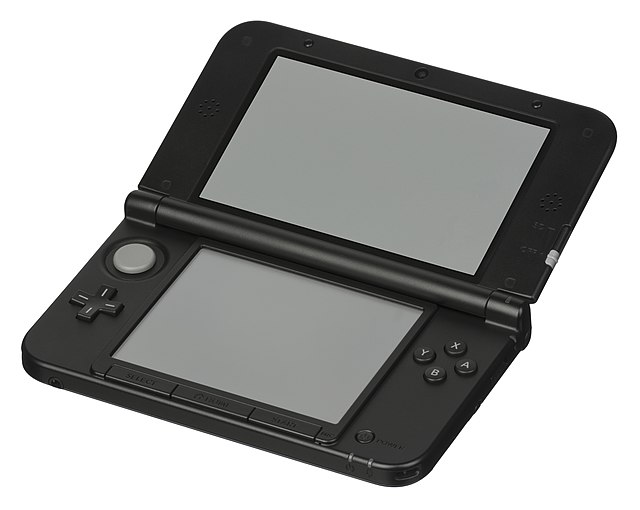
\includegraphics[width=0.5\textwidth]{nintendo_logo.png}
\caption{Nintendo Logo}
\label{fig:nintendo-logo}
\end{figure}

\section{Cultural Impact}

Mario's influence extends beyond games; he has become a cultural icon. From TV shows to merchandise, Mario's presence is ubiquitous\cite{marioCulturalImpact}. The character's universal appeal is a testament to the creativity and vision of Nintendo.

\section{Future Prospects}

Looking ahead, Nintendo continues to innovate with new technologies and gaming experiences. The future holds exciting possibilities for both Mario and Nintendo as they continue to shape the gaming landscape\cite{nintendoFuture}.

\section{Conclusion}

The story of Super Mario and Nintendo is one of creativity, innovation, and enduring success. From their early beginnings to their current status as industry leaders, Mario and Nintendo have left an indelible mark on the world of gaming\cite{marioLegacy}.

\printbibliography

\end{document}

